\section{Section}\label{sse:Section}

\subsection{Subsection}\label{sss:Subsection}

Example citation \citep{baarslag2015learning}

\dfn{Title}{dfnRef}{Definition environment.}

Reference to Definition \ref{dfn:dfnRef}.

\qs{Title}{qsRef}{Question environment.}

\sol{Solution to Question \ref{qs:qsRef}}.

\clm{Title}{clmRef}{Claim environment.}

Reference to Claim \ref{clm:clmRef}

\ex{Title}{exRef}{Example environment.}

Reference to Example \ref{ex:exRef}.

\thm{Title}{thmRef}{Theorem environment.}

\pf{of Theorem \ref{thm:thmRef}}{Proof environment.}

\cor{Title}{corRef}{Corollary environment.}

Reference to Corollary \ref{cor:corRef}.

\lem{Title}{lemRef}{Lemma environment.}

Reference to Lemma \ref{lem:lemRef}.

\prp{Title}{prpRef}{Proposition environment.}

Reference to Proposition \ref{prp:prpRef}.

\begin{figure}[H]
    \centering
    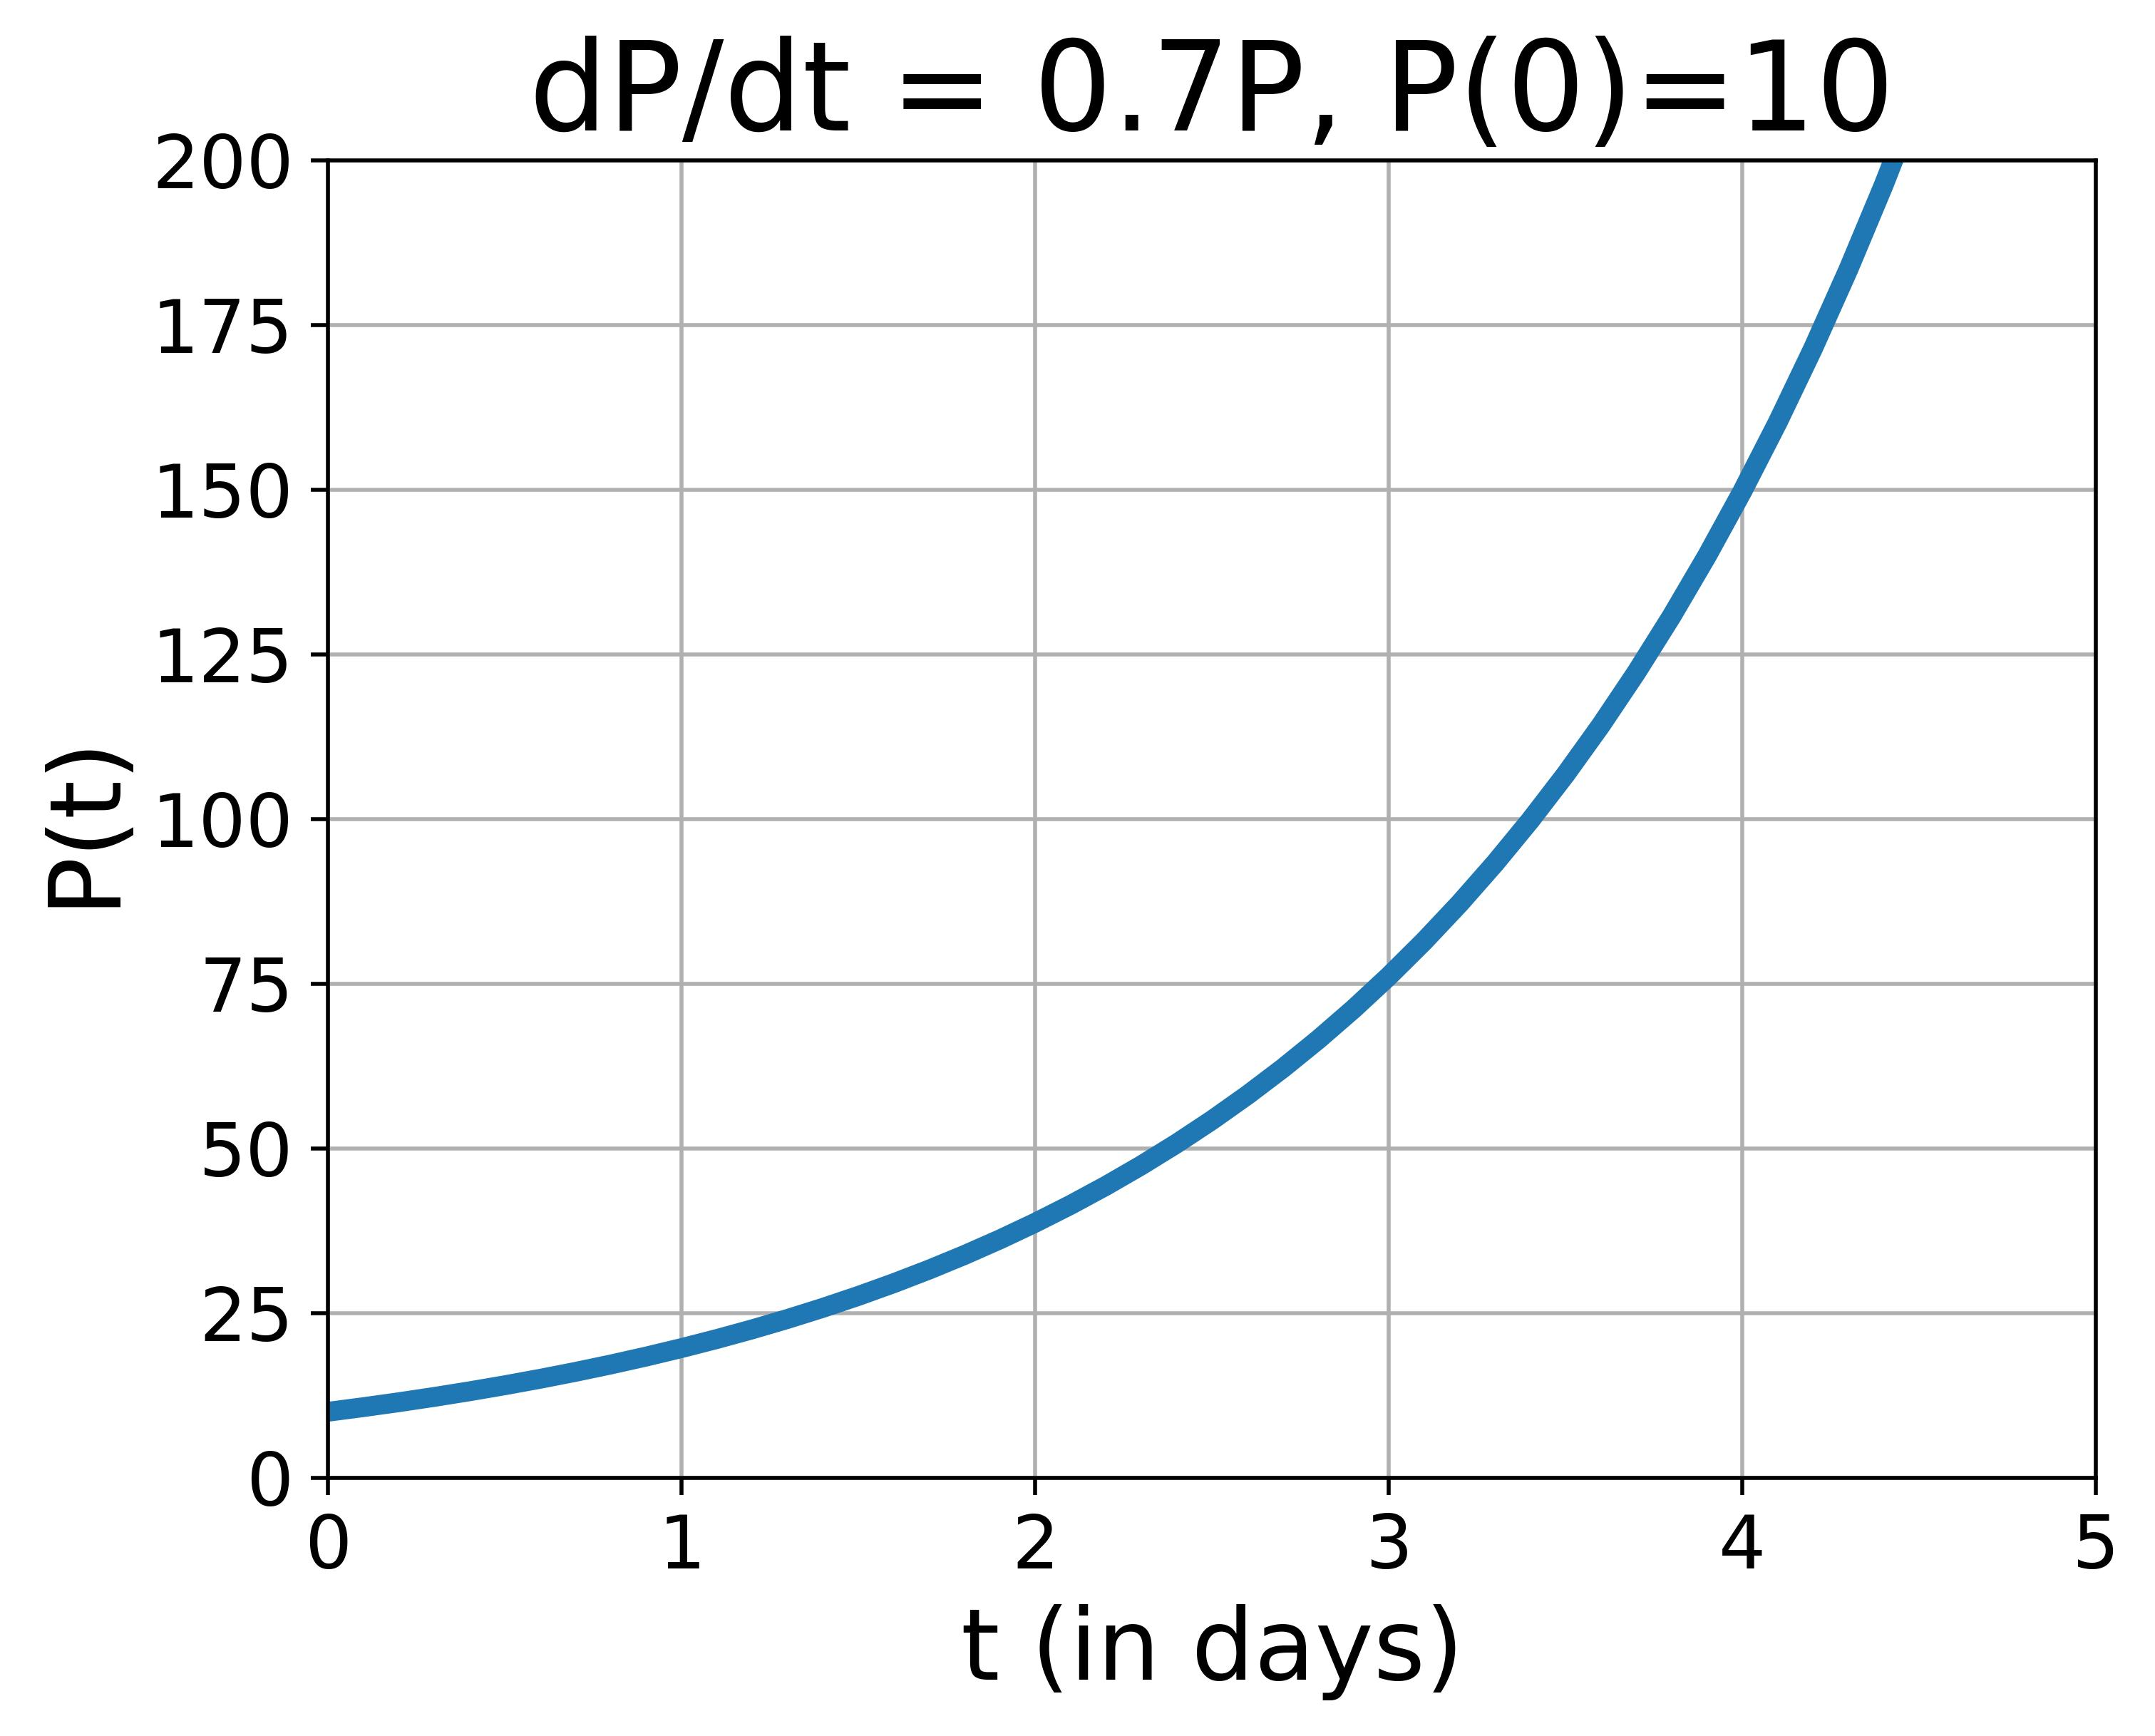
\includegraphics[width=0.6\textwidth]{Rainbowfish.jpg}
    \caption[Rainbowfish population as a function of time]{Rainbowfish population as a function of time.
        This figure is the output of the code in Appendix \ref{app:Example-Python-script}  \citep{tudelftopencourseware}.}
    \label{fig:Rainbowfish}
\end{figure}